\section{Wstęp}
\subsection{Problematyka}
W czasach, w których żyjemy jesteśmy przyzwyczajeni do niemalże natychmiastowego dostępu do informacji. Aby zapewnić ciągły dostęp do informacji, konieczne jest uwzględnienie serwerów, które posiadają dostęp do tych danych. Te serwery często operują w różnych środowiskach uruchomieniowych.

Specjalnie dla sieci \nomrefpage{WWW}, został stworzony język JavaScript, który miał być wykorzystywany w przeglądarkach. Wydajność samego języka na samym początku pozostawiała dużo do życzenia, jednakże obecnie jest zdecydowanie szybszy. Obecnie język stał się językiem ogólnego użytku, jest używany nie tylko do tworzenia interakcji z przeglądarką, także jako serwer wysyłający zapytania \nomrefpage{HTTP} do użytkowników. Badania przeprowadzone przez \cite{comparison_of_servers} wykazują, że Node pozwala na zwiększenie przepustowości serwera, wykorzystując operacje wejścia/wyjścia. W wyżej wymienionych badań wykazano, iż liczba rdzeni ma duży wpływ na wydajność samego serwera, a spowodowane jest to architekturą samego języka oraz braku wielowątkowości języka. 

Twórcy silnika V8, porównują swoją wydajność za pomocą autorskich testów wydajnościowych \cite{ten_years_of_v8_chromium} \cite{ten_years_of_v8}. Testy te są udostępniane również dla innych przeglądarek, co pozwala porównać inne silniki do V8. Test ten określa wydajność za pomocą punktów, które pozwalają ustalić, czy wydajność silnika zmieniła się w przeciągu roku. Rysunek \ref{fig:performance_v8} przedstawia wynik rozwoju silnika na przestrzeni lat 2010-2018.

\begin{figure}[h]
  \centering
  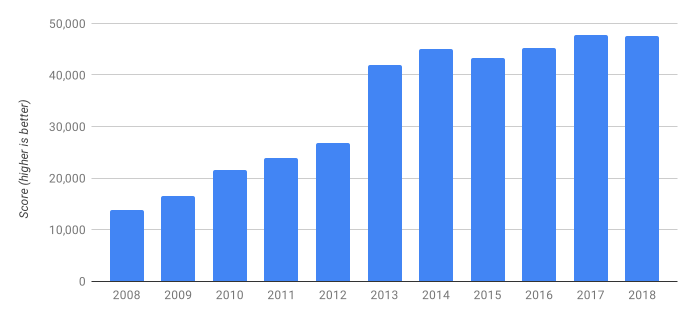
\includegraphics[width=0.9\textwidth]{Figures/v8_bench_2010_2018.png}
  \caption{Wynik przeprowadzonych testów silnika JavaScript 2010-2018 Źródło: \cite{ten_years_of_v8_chromium}}
  \label{fig:performance_v8}
\end{figure}

Na przestrzeni lat środowiskiem, które przodowało i zostało najczęściej adoptowane było, środowisko NodeJS. Tą zależność pokazuje coroczna ankieta \textit{State Of Js} \cite{State_of_js:2021} \cite{State_of_js:2022}, która zbiera wyniki od deweloperów. Deweloperzy odpowiadają, czy znają daną technologię, czy używali jej w przeszłości. W tej ankiecie możemy zauważyć, że na przestrzeni lat pojawili się konkurenci dla NodeJS, tymi alternatywami są Deno i Bun. Jeżeli porównamy wyniki z 2022 roku oraz 2021, możemy zauważyć, że Deno wzmocniło swoją pozycję na rynku. Deweloperzy zaczęli coraz częściej korzystać z nowej technologi. W ankiecie \textit{State Of Js} \cite{State_of_js:2021} \cite{State_of_js:2022} z wymienionych powyżej lat nie możemy jednak otrzymać informacji o środowisku nazwanym Bun, co jest to spowodowane wydaniem wersji 1.0 we wrześniu 2023.

Wymieniona powyżej ankieta mówi tylko o znajomości oraz popularności danego środowiska, aby dowiedzieć się jak dokładnie wygląda praca w danym środowisku musimy wykonać szereg działań, aby przekonać się o jego wydajności. Powstała duża liczba artykułów, które poruszały temat wydajności danego środowiska, jednak nie jesteśmy w stanie stwierdzić, jakie testy przeprowadzili twórców tych artykułów. Dodatkowo nie są one udostępnione dla czytelnika artykułu.

Obecnie, duża ilość aplikacji webowych jest tworzona w języku JavaScript, co pozwala na tworzenie aplikacji zarówno po stronie klienta, jak i serwera. W związku z tym, że język ten jest używany w różnych środowiskach, konieczne jest przeprowadzenie badań, które pozwolą na określenie wydajności danego środowiska. Taka ewaluacja pozwoli na wybór odpowiedniego środowiska do tworzenia aplikacji, które będą wykorzystywane w różnych celach oraz na wskazanie zalet oraz wad danego środowiska, co pozwala na udoskonalenie wydajności środowisk.  

\subsection{Cel pracy}
Celem niniejszej pracy przeprowadzenie badań nt. obecnie występujących środowisk uruchomieniowych oraz analiza zalet oraz wad tych środowisk. W tym celu zidentyfikowano różne środowiska uruchomieniowe, a następnie opracowano zestaw testów wydajnościowych, które pozwoliły na ocenę działania każdego środowiska pod kątem wykorzystywanych algorytmów. Dla przedstawienia wyników testów  została przygotowana aplikacja webowa, której zadaniem jest prezentowanie wyników testów w oparciu o \textit{React} \cite{React} oraz \textit{FastAPI} \cite{FastAPI}. Dla każdego testu zostanie przygotowany wykres z czasami wykonania dla danej iteracji, ilość pamięci wykorzystanej wraz z zużyciem procesora w trakcie wykonywania testu. Dla testu związanego z żądaniami \nomrefeq{HTTP} został rozszerzony o statystyki, które posiada program \textit{oha} \cite{oha}.

\subsection{Zakres pracy}
Zakres pracy obejmuje zbudowanie testów wydajnościowych w językach JavaScript oraz TypeScript dla wybranych środowisk uruchomieniowych JavaScript, przedstawienie wyników testów oraz ich analizę. Umożliwiająca analizę wyników testów została zbudowana aplikacja w oparciu o \textit{React} \cite{React} oraz \textit{FastAPI} \cite{FastAPI} aplikacja webowa, która przestawia dane w formie wykresu wraz z danymi o zużyciu procesora oraz pamięci \nomrefeq{RAM}.

\subsection{Układ pracy}
W tej sekcji znajduje się opis poszczególnych rozdziałów:
\begin{enumerate}
  \item Wstęp - rozdział, który przedstawia problematykę, cel oraz zakres pracy.
  \item Przegląd środowisk uruchomieniowych - rozdział, w którym opisane są wybrane środowiska uruchmomieniowe.
  \item Metodologia badań - rozdział, w którym została przedstawiona metodologia przeprowadzonych badań.
  \item Eksperymenty - rozdział, w którym zostały przedstawione wyniki przeprowadzonych badań.
  \item Dyskusja wyników - rozdział, w którym przedstawiona jest analiza wyników badań.
  \item Podsumowanie - rozdział, w którym zostały przedstawione wnioski dotyczące wyników.
\end{enumerate}
